\chapter[Thème 1 $-$ Continuité d'une fonction]{Thème 1 : Modèles définis par une fonction \\Continuité d'une fonction}
\thispagestyle{fancy}

\section{Notion de continuité}


\begin{bhistoire}
	\begin{minipage}[c]{0.1\linewidth}
		
\includegraphics[scale=0.2]{Img-Cours-01}
	\end{minipage} \hfill
	\begin{minipage}[c]{0.88\linewidth}
		Le mathématicien allemand Karl Weierstrass (1815 ; 1897) apporte les premières définitions rigoureuses au concept de limite et de continuité d'une fonction.
	\end{minipage}
\end{bhistoire}	


\subsection{Définition}

\begin{bdefi}
	\grasInDef{Définition intuitive:}\\
	\phantom{$\dfrac{1}{2}$}\pointilles[\textwidth-0.5cm]
	
	\phantom{$\dfrac{1}{2}$}\pointilles[\textwidth-0.5cm]
\end{bdefi}	

\begin{bmethodet}{Reconnaître graphiquement une fonction continue}
	\grasInMet{Enoncé :}
	
	Étudier graphiquement la continuité des fonctions \(f\) et \(g\) définies et représentées ci-dessous sur l'intervalle [-2;2].\\
	
\includegraphics[scale=0.22]{Img-Cours-02}
	
\includegraphics[scale=0.22]{Img-Cours-03}
	
	\grasInMet{Réponse :}
	
	\begin{itemMet}
		\item \phantom{$\dfrac{1}{2}$}\pointilles[\textwidth-0.5cm]
		\item \phantom{$\dfrac{1}{2}$}\pointilles[\textwidth-0.5cm]
		
		
		\phantom{$\dfrac{1}{2}$}\pointilles[\textwidth-0.5cm]
		
		\phantom{$\dfrac{1}{2}$}\pointilles[\textwidth-0.5cm]
	\end{itemMet}
\end{bmethodet}

\begin{bprop}
	Soit une fonction \(f\) définie sur un intervalle \(I\) contenant un réel \(a\).
	\begin{itemProp}
		\item \phantom{$\dfrac{1}{2}$}\pointilles[\textwidth-0.5cm]
		\item \phantom{$\dfrac{1}{2}$}\pointilles[\textwidth-0.5cm]
	\end{itemProp}
\end{bprop}


\begin{bthm}
	\phantom{$\dfrac{1}{2}$}\pointilles[\textwidth-0.5cm]
\end{bthm}

\begin{bexemples}
	
	
\includegraphics[scale=0.22]{Img-Cours-04}
	
\includegraphics[scale=0.22]{Img-Cours-05}\\
	
\includegraphics[scale=0.22]{Img-Cours-06}
	
\includegraphics[scale=0.22]{Img-Cours-07} 
\end{bexemples}

\subsection{Cas des fonctions de référence}
Les fonctions suivantes sont continues sur l'intervalle donné.

\begin{center}
	\begin{tabular}{|c|c|}
		\hline
		Fonction & Intervalle \\
		\hline
		\(|x|\) & \(\mathbb{R}\) \\
		\hline
		\(x^{n}(n \in \mathbb{N})\) & \(\mathbb{R}\) \\
		\hline
		Polynôme & \(\mathbb{R}\) \\
		\hline
		\(e^{x}\) & \(\mathbb{R}\) \\
		\hline
		\(\sqrt{x}\) & \([0 ;+\infty[\) \\
		\hline
		\(\dfrac{1}{x}\) & \(]-\infty ; 0[\) et \(] 0 ;+\infty[\) \\
		\hline
	\end{tabular}
\end{center}

\subsection{Opérations sur les fonctions continues:}

\begin{bprops}
	
\(f\) et \(g\) sont deux fonctions continues sur un intervalle \(I\).

\begin{itemProp}
	\item \phantom{$\dfrac{1}{2}$}\pointilles[\textwidth-0.5cm]
	\item \phantom{$\dfrac{1}{2}$}\pointilles[\textwidth-0.5cm]
\end{itemProp}

\end{bprops}

\begin{brmq}
Dans la pratique, les flèches obliques d'un tableau de variations traduisent la continuité et la stricte monotonie de la fonction sur l'intervalle considéré.
\end{brmq}

\begin{bmethodet}{Étudier la continuité d'une fonction définie par morceaux}
	\grasInMet{Enoncé :}
	
	On considère la fonction \(f\) définie sur \(\mathbb{R}\) par \(f(x)=\left\{\begin{array}{l}-x+2, \text { pour } x<3 \\ x-4, \text { pour } 3 \leq x<5 \\ -2 x+13, \text { pour } x \geq 5\end{array}\right.\)\\
	La fonction \(f\) est-elle continue sur \(\mathbb{R}\) ?
	
	\grasInMet{Réponse :}
	
	Les fonctions \(x \mapsto-x+2, x \mapsto x-4\) et \(x \mapsto-2 x+13\) sont des fonctions polynômes donc continues sur \(\mathbb{R}\).\\
	Ainsi la fonction \(f\) est continue sur \(]-\infty ; 3[\), sur \([3 ; 5[\) et sur \([5 ;+\infty[\).\\
	Étudions alors la continuité de \(f\) en 3 et en 5 :
	
	\begin{itemMet}
		\item \phantom{$\dfrac{1}{2}$}\pointilles[\textwidth-0.5cm]
		
		\phantom{$\dfrac{1}{2}$}\pointilles[\textwidth-0.5cm]
		
		\phantom{$\dfrac{1}{2}$}\pointilles[\textwidth-0.5cm]
		
		\phantom{$\dfrac{1}{2}$}\pointilles[\textwidth-0.5cm]
		\item \phantom{$\dfrac{1}{2}$}\pointilles[\textwidth-0.5cm]
		
		\phantom{$\dfrac{1}{2}$}\pointilles[\textwidth-0.5cm]
		
		\phantom{$\dfrac{1}{2}$}\pointilles[\textwidth-0.5cm]
		
		\phantom{$\dfrac{1}{2}$}\pointilles[\textwidth-0.5cm]
		
		\phantom{$\dfrac{1}{2}$}\pointilles[\textwidth-0.5cm]
		
		\phantom{$\dfrac{1}{2}$}\pointilles[\textwidth-0.5cm]
	\end{itemMet}
	
	En représentant la fonction \(f\), on peut observer graphiquement le résultat précédent.
	\begin{center}
		
\includegraphics[scale=0.16]{Img-Cours-08}
	\end{center}
	
\end{bmethodet}



\section{Théorème des valeurs intermédiaires}

\begin{bexemple}
	On donne le tableau de variations de la fonction \(f\).
	
	\begin{center}
		\begin{tikzpicture}
			\tkzTabInit{$x$ / 1 , $f(x)$ / 1.5}{$-4$, $-3$, $-1$, $1$}
			\tkzTabVar{-/ $-1$, +/ $3$, -/ $-1$, +/ $19$}
		\end{tikzpicture}
	\end{center}
	
	Il est possible de lire dans le tableau, le nombre de solutions éventuelles pour des équations du type \(f(x)=k\) :
	
	\begin{itemEx}
		\item L'équation \(f(x)=18\) possède 1 solution comprise dans l'intervalle \(]-1 ; 1[\).
		\item L'équation \(f(x)=0\) possède 3 solutions chacune comprise dans un des intervalles ]-4 ; \(-3[]-,3 ;-1[\) et \(]-1 ; 1[\).
		\item L'équation \(f(x)=-3\) ne possède pas de solution.
		\item L'équation \(f(x)=3\) possède 2 solutions : I'une égale à -3 , l'autre comprise dans l'intervalle ]-1 ; 1[.
	\end{itemEx}
\end{bexemple}

\begin{bthm}


\grasInProp{Théorème des valeurs intermédiaires :}

On considère la fonction \(f\) continue sur l'intervalle \([a ; b]\).
\begin{itemProp}
	\item \phantom{$\dfrac{1}{2}$}\pointilles[\textwidth-0.5cm]
	
	\phantom{$\dfrac{1}{2}$}\pointilles[\textwidth-0.5cm]
	
	
\includegraphics[scale=0.23]{Img-Cours-09}
	\item \phantom{$\dfrac{1}{2}$}\pointilles[\textwidth-0.5cm]
	
	\phantom{$\dfrac{1}{2}$}\pointilles[\textwidth-0.5cm]
	
	
\includegraphics[scale=0.25]{Img-Cours-10}
\end{itemProp}

\end{bthm}

\begin{bmanip}
	Dans la pratique:
	
	Pour démontrer que l'équation \(f(x)=0\) admet une unique solution sur l'intervalle \([a ; b]\), on démontre que :
	
	\begin{enumMet}
		\item \phantom{$\dfrac{1}{2}$}\pointilles[\textwidth-0.5cm]
		\item \phantom{$\dfrac{1}{2}$}\pointilles[\textwidth-0.5cm]
		\item \phantom{$\dfrac{1}{2}$}\pointilles[\textwidth-0.5cm]
	\end{enumMet}
	
	Les conditions 1 et 2 nous assurent que des solutions existent.\\
	Avec la condition 3 en plus, nous savons que la solution est unique.
	
\end{bmanip}

\begin{bmethodet}{Appliquer le théorème des valeurs intermédiaires (1)}
	\grasInMet{Enoncé :}
	
	On considère la fonction \(f\) définie sur \(\mathbb{R}\) par \(f(x)=x^{3}-x^{2}-1\).
	
	\begin{enumMet}
		\item Démontrer que l'équation \(f(x)=0\) admet une unique solution \(\alpha\) sur l'intervalle [ \(1 ; 2\) ].
		\item À l'aide de la calculatrice, donner un encadrement au centième de la solution \(\alpha\).
	\end{enumMet}
	
	\grasInMet{Réponse :}
	
	\begin{enumMet}
		\begin{minipage}[c]{0.68\linewidth}
			\item \begin{itemMet}
			\item \phantom{$\dfrac{1}{2}$}\pointilles[\textwidth-0.5cm]
			
			\phantom{$\dfrac{1}{2}$}\pointilles[\textwidth-0.5cm]
			\item \phantom{$\dfrac{1}{2}$}\pointilles[\textwidth-0.5cm]
			
			\phantom{$\dfrac{1}{2}$}\pointilles[\textwidth-0.5cm]
			
			\phantom{$\dfrac{1}{2}$}\pointilles[\textwidth-0.5cm]
			
			\phantom{$\dfrac{1}{2}$}\pointilles[\textwidth-0.5cm]
			\item \phantom{$\dfrac{1}{2}$}\pointilles[\textwidth-0.5cm]
			
			\phantom{$\dfrac{1}{2}$}\pointilles[\textwidth-0.5cm]
			
			\phantom{$\dfrac{1}{2}$}\pointilles[\textwidth-0.5cm]
			
			\phantom{$\dfrac{1}{2}$}\pointilles[\textwidth-0.5cm]
		\end{itemMet}
		
		\phantom{$\dfrac{1}{2}$}\pointilles[\textwidth-0.5cm]
		
		\phantom{$\dfrac{1}{2}$}\pointilles[\textwidth-0.5cm]
		
		\phantom{$\dfrac{1}{2}$}\pointilles[\textwidth-0.5cm]
		\end{minipage} \hfill
		\begin{minipage}[c]{0.28\linewidth}
			
\includegraphics[scale=0.25]{Img-Cours-11}
		\end{minipage}
		\item A l'aide de la calculatrice, il est possible d'effectuer des \guillemets{balayages successifs} en augmentant la précision.
		
		\begin{minipage}[c]{0.48\linewidth}
			La solution est comprise entre 1,4 et 1,5.
			
			En effet : \(f(1,4) \approx-0,216<0\)
			
			\(f(1,5) \approx 0,125>0\)
		\end{minipage} \hfill
		\begin{minipage}[c]{0.48\linewidth}
			
\includegraphics[scale=0.75]{Img-Cours-12}
		\end{minipage}
		
		\begin{minipage}[c]{0.48\linewidth}
			La solution est comprise entre 1,46 et 1,47.
			
			En effet : \(f(1,46) \approx-0,019<0\)
			
			\(f(1,47) \approx 0,0156>0\)
			
			On en déduit que : \(1,46<\alpha<1,47\).
		\end{minipage} \hfill
		\begin{minipage}[c]{0.48\linewidth}
			
\includegraphics[scale=0.75]{Img-Cours-13}
		\end{minipage}

	\end{enumMet}
	
\end{bmethodet}

\begin{bmethodet}{Appliquer le théorème des valeurs intermédiaires (2)}
	\grasInMet{Enoncé :}
	
	On considère la fonction \(f\) définie sur \(\mathbb{R}\) par \(f(x)=x^{3}-4 x^{2}+6\).\\
	Démontrer que l'équation \(f(x)=2\) admet au moins une solution sur \([-1 ; 4]\).
	
	
	\grasInMet{Réponse :}
	
	\begin{itemMet}
		\item \phantom{$\dfrac{1}{2}$}\pointilles[\textwidth-0.5cm]
		
		\phantom{$\dfrac{1}{2}$}\pointilles[\textwidth-0.5cm]
		
		\item \phantom{$\dfrac{1}{2}$}\pointilles[\textwidth-0.5cm]
		
		\phantom{$\dfrac{1}{2}$}\pointilles[\textwidth-0.5cm]
		
		\phantom{$\dfrac{1}{2}$}\pointilles[\textwidth-0.5cm]
		
		\phantom{$\dfrac{1}{2}$}\pointilles[\textwidth-0.5cm]
		
		\phantom{$\dfrac{1}{2}$}\pointilles[\textwidth-0.5cm]
		
		\phantom{$\dfrac{1}{2}$}\pointilles[\textwidth-0.5cm]
	\end{itemMet}

\begin{brmq}
	Ici, on n'a pas la stricte monotonie de \(f\), donc on n'a pas l'unicité de la solution.
\end{brmq}
	
\end{bmethodet}
    


